\documentclass[10pt, a4paper]{report}

\usepackage[utf8]{inputenc}
\usepackage{polski}
\usepackage{a4wide}
\usepackage{fancyhdr}
\usepackage{lastpage}
\usepackage{tabularx}
\usepackage{graphicx}
\usepackage{listings}

\graphicspath{ {./images} }

%strona tytułowa
\begin{titlepage}

\title{\huge{\textbf{Specyfikacja implementacyjna} \\ programu grapher}}
\author{Szymon Półtorak i Sebastian Sikorski}
\date{17.03.2022r}

\end{titlepage}

\renewcommand{\footrulewidth}{1pt}

\begin{document}
    \maketitle

    %poprawa numeracji sekcji z 0.* na *
    \renewcommand*\thesection{\arabic{section}} 

    %druga strona (streszczenie)
    \begin{abstract}
        W dokumencie zawarte są informacje na temat implementacji projektu dotyczącego \textit{grafów}, napisanego w języku \textit{C}.
        Przedstawiane są metody implementacji, podział na moduły, środowisko w jakim program został napisany oraz wyjaśnione jest jego działanie.
    \end{abstract}
    
    %numerowanie stron
    \pagestyle{fancy}
    \fancyhf{}
    \lhead{Specyfikacja implementacyjna programu \textit{grapher}(C)}
    \rhead{Szymon Półtorak i Sebastian Sikorski}
    \cfoot{Strona \thepage \hspace{1pt} z \pageref{LastPage}}
    
    %spis treści
    \fancypagestyle{plain}{
        \lhead{Specyfikacja implementacyjna programu \textit{grapher}(C)}
        \rhead{Szymon Półtorak i Sebastian Sikorski}
        \cfoot{Strona \thepage \hspace{1pt} z \pageref{LastPage}}
    }
    \tableofcontents
    \newpage

    \section{Cel projektu - streszczenie}
    Program ma za zadanie generować pliki z grafami o ustalonym formacie oraz czytanie takich plików w celu znalezienia najkrótszej ścieżki między podanymi
    przez użytkownika punktami. Grapher posiada cztery tryby:
    \begin{itemize}
        \item Wage Mode – program generuje graf spójny o losowych wagach krawędzi,
        \item Edge Mode – program losuje istnienie krawędzi między wierzchołkami grafu oraz wagi do
        momentu powstania grafu spójnego,
        \item Random Mode – program losuje istnienie krawędzi i ich wagi. W tym trybie graf może być niespójny,
        \item Read Mode – program czyta plik o ustalonym formacie i szuka drogi pomiędzy podanymi przez użytkownika punktami.        
    \end{itemize}
    Po szczegółowe wyjaśnienie funkcjonalności trybów, formatu pliku z grafem, struktury folderu oraz składni programu odsyłamy do specyfikacji funkcjonalnej projektu \textit{grapher}.

    \section{Środowisko pracy}
    \begin{tabularx}{\textwidth}{ X|X }
        \hline Język programowania & C17 (ISO/IEC 9899:2018) \\
        \hline Kompilator & gcc 10.2.1 \\
        \hline System Operacyjny & Windows Subsystem for Linux, Debian 11 \\
        \hline Środowisko programistyczne & Visual Studio Code 1.65.2 \\
        \hline System kontroli wersji & Git 2.30.2 \\
        \hline
    \end{tabularx}

    \section{Diagram modułów}
    Program składa się z trzech modułów: \texttt{genGraph}, \texttt{alloc} i \texttt{readGraph}. Składają się one z dwóch plików każdy. Jednym z nich jest plik źródłowy \textit{.c}, a drugi to plik nagłówkowy \textit{.h}.
    Oprócz nich znajduje się również plik \texttt{main.c}, zawierający główną funkcję sterującą programem.
    \begin{figure}[h]
        \begin{center}
            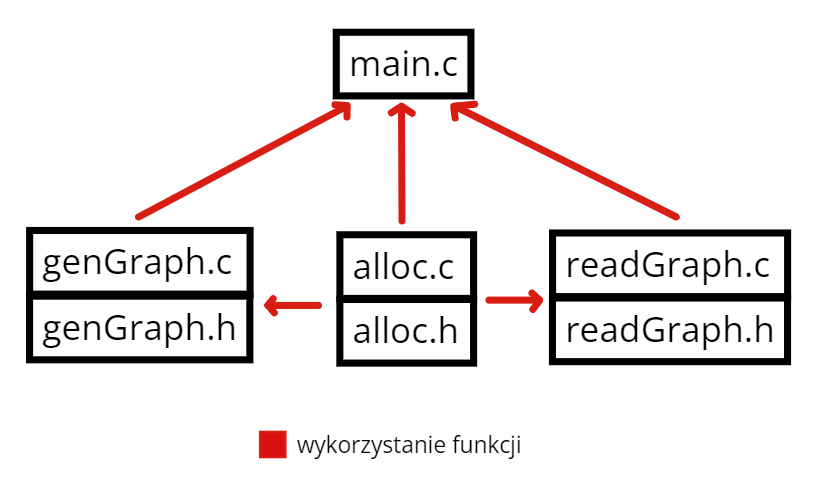
\includegraphics[scale=0.5]{modules_diagram.jpg}
            \caption{Diagram modułów.}
        \end{center}        
    \end{figure}
    \newpage

    \section{Przedstawienie poszczególnych modułów}
    Plik \texttt{main.c} odpowiada za sterowanie całym programem i wywołuje potrzebne funkcje z odpowiednich modułów.
    Moduły programu i ich rola:
    \begin{itemize}
        \item \textbf{Moduł alloc} -- znajdują się w nim funkcje pomogające programowi w alokowaniu i uwalnianiu pamięci z tablic i struktur,
        \item \textbf{Moduł genGraph} -- zawiera on funkcje odpowiedzialne za generowanie grafu w trzech trybach oraz funkcje pomagające wykonanie odpowiednich procedur w danym trybie,
        \item \textbf{Moduł readGraph} -- posiada on funkcje, których zadaniem jest wczytywanie grafu, sprawdzanie jego spójności oraz znajdowanie w nim najkrótszej ściężki między zadanymi punktami.
    \end{itemize}

    \section{Wykorzystane algorytmy}

    \subsection{Breadth-first search(BFS)}
    Sprawdzanie spójności grafu rozpoczyna się z dowolnego wierzchołka, w przypadku naszego algorytmu domyślnym wierzchołkiem jest wierzchołek zero. 
    Algorytm w celu sprawdzenia spójności tworzy tablicę poprzedników o długości odpowiadającej ilości wierzchołków oraz zapełnia ją wartościami -1. 
    Rozpoczynając iteracje od wierzchołka zero aż do ostatniego wierzchołka.
    Algorytm sprawdza z jakimi wierzchołkami połączony jest obecny i dopisuje te wierzchołki do kolejki typu \textit{FIFO}, czyli kolejka typu \textit{first in first out}, czyli pierwszy wchodzi i wychodzi 
    , jednocześnie uzupełniając tablicę poprzedników. 
    Po takim kroku algorytm przechodzi do kolejnego wierzchołka pobierając jego \textit{ID} z kolejki.
    Przy dotarciu do końca kolejki algorytm musi sprawdzić czy jednym wierzchołkiem bez poprzednika jest wierzchołek zero, w przeciwnym przypadku test spójności jest negatywny.
    \begin{figure}[h]
        \begin{center}
            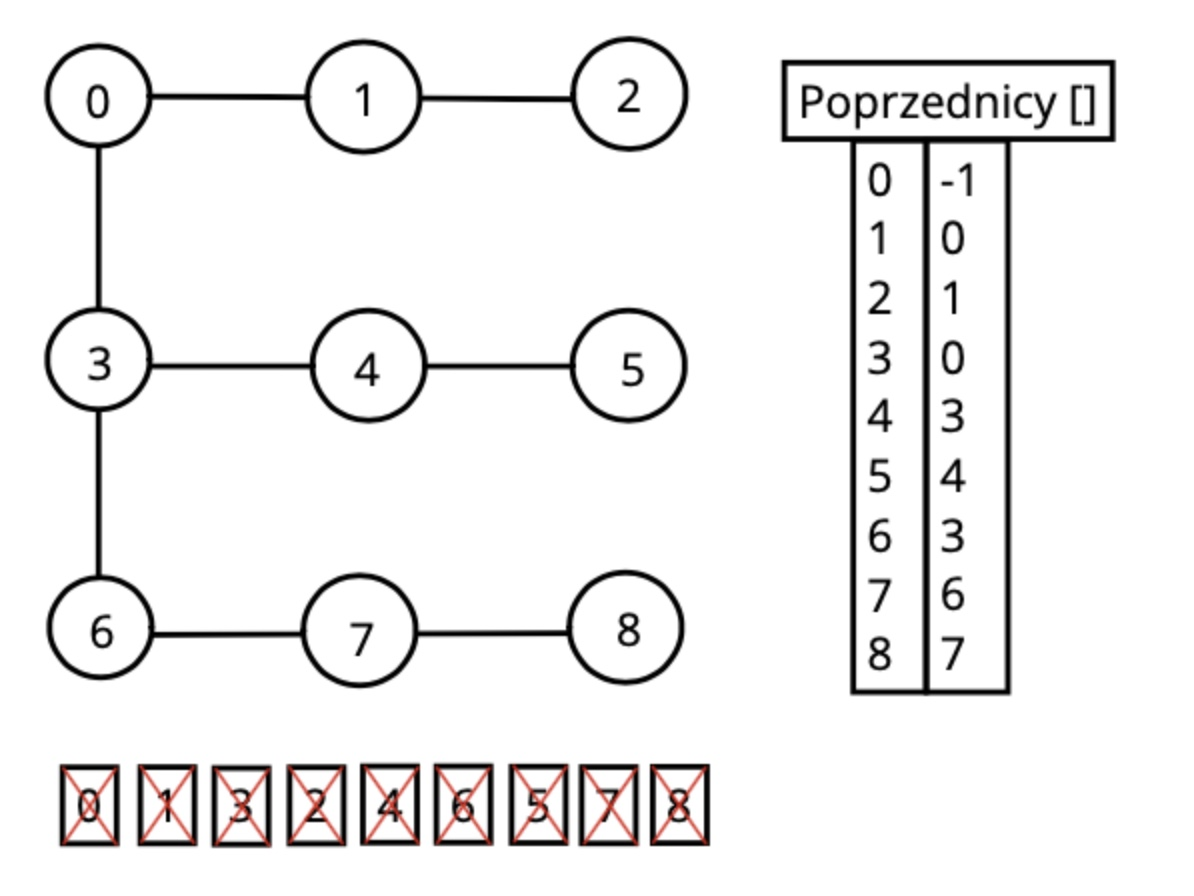
\includegraphics[scale=0.2]{bfs_example.jpg}
            \caption{Przykładowy graf wraz z tablicą poprzedników.}
        \end{center}        
    \end{figure}    
    \newpage

    \subsection{Algorytm Dijkstry}
    Algorytm Dijkstry liczy najkrótszą odległość od wierzchołka początkowego do wszystkich innych wierzchołków, ale w naszej implementacji skupiamy się jedynie na najkrótszej ścieżce między wierzchołkami zadanymi przez użytkownika. 
    Algorytm ten korzysta z trzech tablic przechowujących informacje odpowiednio o tym czy wierzchołek odwiedzono, dystansie jakiego dotąd wymagało odwiedzenie oraz poprzedniku tego odwiedzenia.
    W przeciwieństwie do algorytmu BFS, algorytm ten korzysta z kolejki priorytetowej, gdzie wartością decydującą jest dotychczasowa odległość do punktu. Dalej analogicznie następuje iterowanie po wszystkich wierzchołkach 
    aż do momentu, w~którym kolejka jest pusta. Następnie zaczynając od wierzchołka końcowego (podanego przez użytkownika) cofamy się aż trafimy do wierzchołka początkowego. 
    Podczas cofania zapisujemy przez jakie wierzchołki przeszliśmy oraz jaka była waga takiego przejścia.
    \begin{figure}[h]
        \begin{center}
            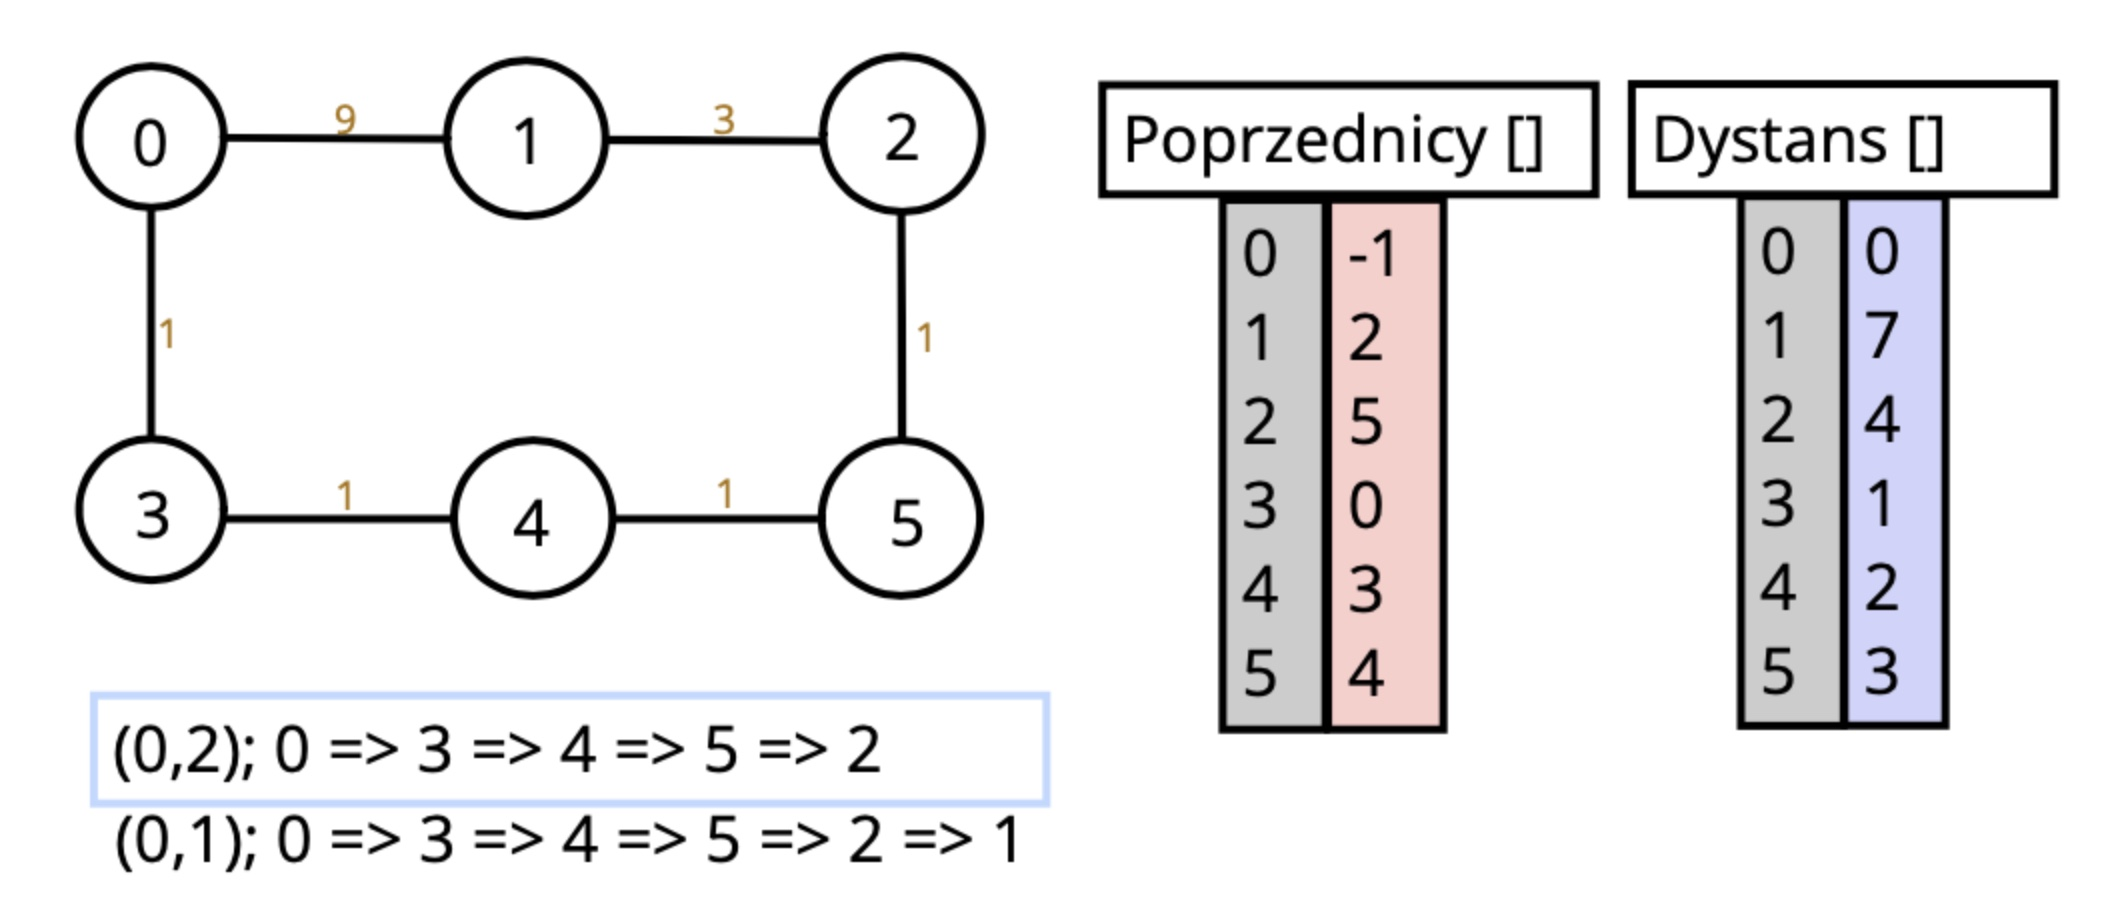
\includegraphics[scale=0.15]{dijkstra_example.jpg}
            \caption{Przykładowy wynik najkrótszej ścieżki w algorytmie Dijkstry.}
        \end{center}        
    \end{figure}

    \section{Wykorzystane struktury}
    Poniżej prezentujemy najważniejsze struktury wykorzystane przez nasz program:
    \begin{itemize}
        \item \texttt{struct entryRead}:
        \begin{lstlisting}
struct entryRead {
    char* fileName;
    bool printFlag;
    int* points;
} entryR;
        \end{lstlisting}
        \item \texttt{struct entryGen}:
        \begin{lstlisting}
struct entryGen {
    int rows;
    int columns;
    double rangeStart;
    double rangeEnd;
    short int mode;
    char* fileName;
} entryG;
        \end{lstlisting}
        \newpage
        \item \texttt{struct node}:
        \begin{lstlisting}
struct node {
    bool* edgeExist;
    double* edgeWeight;
} node;
        \end{lstlisting}
        \item \texttt{struct graphRead}:
        \begin{lstlisting}
struct graphRead {
    node** graph;
    int rows;
    int columns;
} graphR;
        \end{lstlisting}
    \end{itemize}

    \section{Wykorzystane funkcje}
    W naszym programie zaimplementowane zostało wiele funkcji oraz struktur. Poniżej prezentujemy tylko te najważniejsze z nich:
    \subsection{Moduł genGraph}
    \begin{itemize}
        \item \texttt{void generateMode(struct entryGen)} -- funkcja główna odpowiadająca za generowanie grafu w wybranym przez użytkownika trybie,
        \item \texttt{bool checkIfCoherentGen(node** graph, entryG* entry)} -- zwraca wartość false lub true w~ zależności, czy graf jest spójny, czy nie,
        \item \texttt{void saveGraphToFile(entryG* entry, node** graph)} -- odpowiada za zapisanie gotowego grafu do pliku,
        \item \texttt{double generateWeights(entryG* entry)} -- jej zadaniem jest wygenerowanie wagi z podanego przez użytkownika przedziału,
    \end{itemize}

    \subsection{Moduł alloc}
    \begin{itemize}
        \item \texttt{entryG* allocEntryGen(char **argv)} -- zwraca wskaźnik na strukturę typu \texttt{entryG},
        \item \texttt{entryR* allocEntryRead(int argc, char **argv)} -- funkcja zwraca wskaźnik na strukturę typu \texttt{entryR},
    \end{itemize}

    \subsection{Moduł readGraph}
    \begin{itemize}
        \item \texttt{void readMode(struct entryRead)} -- funkcja główna odpowiadjąca za odczytanie pliku i~ znalezienie najkrótszej ścieżki między podanymi przez użytkownika punktami,
        \item \texttt{graphR** readFromFile(entryR* entry)} -- wczytuje graf z odpowiednio sformatowanego pliku do tablicy,
        \item \texttt{int checkIfCoherentRead(graphR** graph, entryR* entry)} -- zwraca wartość 0 lub 1 w zależności, czy graf jest spójny, czy nie,
        \item \texttt{void findPath(graphR** graph, entryR* entry)} -- odpowiada za znalezienie najkrótszej ścieżki między podanymi przez użytkownika punktami,
        \item \texttt{void printShortPath(entryR* entry, int* parents)} -- wyświetla najkrótszą ścieżkę w~ podstawowym formacie,
        \item \texttt{void printExtendedPath(entryR* entry, int* parents, double* weights)} -- wyświetla najkrótszą ścieżkę w rozszerzonym formacie,

    \end{itemize}

    \section{Przeprowadzanie zmian oraz testów}
    Do pracy z projektem wykorzystujemy system kontroli wersji \textit{git}. Wszelkie zmiany w programie będą przekazywane do platformy
    Projektor za pośrednictwem systemu kontroli wersji w postaci commitów. Testowanie programu będzie przeprowadzone w sposób półautomatyczny.
    Do tego będziemy wykorzystywać odpowiednią formułę z pliku \textit{makefile}. 
    Formuła to:
    \begin{itemize}
        \item \textbf{make test} -- formuła odpowiedzialna za skompliowanie plików z folderu test oraz plików bedących modułami w programie grapher. Dokonuje ona komplacji do pliku wykonywalnego \texttt{./test}, a następnie go uruchamia.
    \end{itemize}
  

\end{document}